% \chapter{Některé příkazy balíčku \texttt{thesis}}

% \section{Příkazy pro sazbu veličin a~jednotek}

% \begin{table}[!h]
%   \caption[Přehled příkazů]{Přehled příkazů pro matematické prostředí }
%   \begin{center}
%   	\small
% 	  \begin{tabular}{|c|c|c|c|}
% 	    \hline
% 	    Příkaz    						& Příklad 					& Zdroj příkladu  							& Význam  \\
% 	    \hline\hline
% 	    \verb|\textind{...}|	& $\beta_\textind{max}$ 	& \verb|$\beta_\textind{max}$|	& textový index \\
% 	    \hline
% 	    \verb|\const{...}| 		& $\const{U}_\textind{in}$ 				& \verb|$\const{U}_\textind{in}$|		& konstantní veličina \\
% 	    \hline
% 	    \verb|\var{...}| 		& $\var{u}_\textind{in}$ & \verb|$\var{u}_\textind{in}$| & proměnná veličina \\
% 	    \hline
% 	    \verb|\complex{...}| 	& $\complex{u}_\textind{in}$ & \verb|$\complex{u}_\textind{in}$| & komplexní veličina \\
% 	    \hline
% 	    \verb|\vect{...}| 		& $\vect{y}$ 						& \verb|$\vect{y}$| & vektor \\
% 	    \hline
% 	    \verb|\mat{...}| 	& $\mat{Z}$ 						& \verb|$\mat{Z}$| & matice \\
% 	    \hline
% 	    \verb|\unit{...}| 		& $\unit{kV}$ 						& \verb|$\unit{kV}$|\quad či\ \, \verb|\unit{kV}| & jednotka \\
% 	    \hline
% 	  \end{tabular}
%   \end{center}
% \end{table}



% %\newpage
% \section{Příkazy pro sazbu symbolů}

% \begin{itemize}
%   \item
%     \verb|\E|, \verb|\eul| -- sazba Eulerova čísla: $\eul$,
%   \item
%     \verb|\J|, \verb|\jmag|, \verb|\I|, \verb|\imag| -- sazba imaginární jednotky: $\jmag$, $\imag$,
%   \item
%     \verb|\dif| -- sazba diferenciálu: $\dif$,
%   \item
%     \verb|\sinc| -- sazba funkce: $\sinc$,
%   \item
%     \verb|\mikro| -- sazba symbolu mikro stojatým písmem%
% 			\footnote{znak pochází z~balíčku \texttt{textcomp}}: $\mikro$,
% 	\item
% 		\verb|\uppi| -- sazba symbolu $\uppi$
% 			(stojaté řecké pí, na rozdíl od \verb|\pi|, což sází $\pi$).
% \end{itemize}
% %
% Všechny symboly jsou určeny pro matematický mód, vyjma \verb|\mikro|, jenž je\\ použitelný rovněž v~textovém módu.
% %$\upmikro$


% \chapter{Druhá příloha}

% \begin{figure}[!h]
%   \begin{center}
%     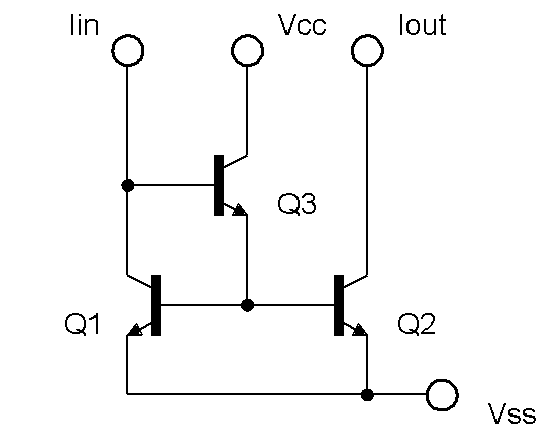
\includegraphics[scale=0.5]{obrazky/ZlepseneWilsonovoZrcadloNPN}
%   \end{center}
%   \caption[Alenčino zrcadlo]{Zlepšené Wilsonovo proudové zrcadlo.}
% \end{figure}

% Pro sazbu vektorových obrázků přímo v~\LaTeX{}u je možné doporučit balíček \href{https://www.ctan.org/pkg/pgf}{\texttt{TikZ}}.
% Příklady sazby je možné najít na \href{http://www.texample.net/tikz/examples/}{\TeX{}ample}.
% Pro vyzkoušení je možné použít programy QTikz nebo TikzEdt.




% \chapter{Příklad sazby zdrojových kódů}

% \section{Balíček \texttt{listings}}

% Pro vysázení zdrojových souborů je možné použít balíček \href{https://www.ctan.org/pkg/listings}{\texttt{listings}}.
% Balíček zavádí nové prostředí \texttt{lstlisting} pro sazbu zdrojových kódů, jako například:
% %
% \begin{lstlisting}[language={[LaTeX]TeX}]
% \section{Balíček lstlistings}
% Pro vysázení zdrojových souborů je možné použít
% 	balíček \href{https://www.ctan.org/pkg/listings}%
% 	{\texttt{listings}}.
% Balíček zavádí nové prostředí \texttt{lstlisting} pro
% 	sazbu zdrojových kódů.
% \end{lstlisting}
% %
% Podporuje množství programovacích jazyků.
% Kód k~vysázení může být načítán přímo ze zdrojových souborů.
% Umožňuje vkládat čísla řádků nebo vypisovat jen vybrané úseky kódu.
% Např.:

% \noindent
% Zkratky jsou sázeny v~prostředí \texttt{acronym}:
% \label{lst:zkratky}
% \lstinputlisting[language={[LaTeX]TeX},nolol,numbers=left, firstnumber=6, firstline=6,lastline=6]{text/zkratky.tex}
% %
% Šířka textu volitelného parametru \verb|KolikMista| udává šířku prvního sloupce se zkratkami.
% Proto by měla být zadávána nejdelší zkratka nebo symbol.
% Příklad definice zkratky \acs{symfvz} je na výpisu \ref{lst:symfvz}.

% \shorthandoff{-}
% \lstinputlisting[language={[LaTeX]TeX},frame=single,caption={Ukázka sazby zkratek},label=lst:symfvz,numbers=left,linerange={bsymfvz-\%\%\%\ esymfvz},includerangemarker=false]{text/zkratky.tex}
% \shorthandon{-}

% \noindent
% Ukončení seznamu je provedeno ukončením prostředí:
% \lstinputlisting[language={[LaTeX]TeX},nolol,numbers=left,firstnumber=26,linerange=26]{text/zkratky.tex}

% \vspace{\fill}

% \noindent
% {\bf Poznámka k~výpisům s~použitím volby jazyka \verb|czech| nebo \verb|slovak|:}\newline
% Pokud Váš zdrojový kód obsahuje znak spojovníku \verb|-|, pak překlad může skončit chybou.
% Ta je způsobená tím, že znak \verb|-| je v~českém nebo slovenském nastavení balíčku \verb|babel| tzv.\ aktivním znakem.
% Přepněte znak \verb|-| na neaktivní příkazem \verb|\shorthandoff{-}| těsně před výpisem a~hned za ním jej vraťte na aktivní příkazem \verb|\shorthandon{-}|.
% Podobně jako to je ukázáno ve zdrojovém kódu šablony.


% \clearpage

% %\section{Výpis kódu prostředí Matlab}
% Na výpisu \ref{lst:priklad.vypis.kodu.Matlab} naleznete příklad kódu pro Matlab, na výpisu \ref{lst:priklad.vypis.kodu.C} zase pro jazyk~C.

% \lstnewenvironment{matlab}[1][]{%
% \iflanguage{czech}{\shorthandoff{-}}{}%
% \iflanguage{slovak}{\shorthandoff{-}}{}%
% \lstset{language=Matlab,numbers=left,#1}%
% }{%
% \iflanguage{slovak}{\shorthandon{-}}{}%
% \iflanguage{czech}{\shorthandon{-}}{}%
% }

% \begin{matlab}[frame=single,float=htbp,caption={Příklad Schur-Cohnova testu stability v~prostředí Matlab.},label=lst:priklad.vypis.kodu.Matlab,numberstyle=\scriptsize, numbersep=7pt]
% %% Priklad testovani stability filtru

% % koeficienty polynomu ve jmenovateli
% a~= [ 5, 11.2, 5.44, -0.384, -2.3552, -1.2288];
% disp( 'Polynom:'); disp(poly2str( a, 'z'))

% disp('Kontrola pomoci korenu polynomu:');
% zx = roots( a);
% if( all( abs( zx) < 1))
%     disp('System je stabilni')
% else
%     disp('System je nestabilni nebo na mezi stability');
% end

% disp(' '); disp('Kontrola pomoci Schur-Cohn:');
% ma = zeros( length(a)-1,length(a));
% ma(1,:) = a/a(1);
% for( k~= 1:length(a)-2)
%     aa = ma(k,1:end-k+1);
%     bb = fliplr( aa);
%     ma(k+1,1:end-k+1) = (aa-aa(end)*bb)/(1-aa(end)^2);
% end

% if( all( abs( diag( ma.'))))
%     disp('System je stabilni')
% else
%     disp('System je nestabilni nebo na mezi stability');
% end
% \end{matlab}

% \noindent
% \begin{minipage}{\linewidth}


% %\section{Výpis kódu jazyka C}

% \begin{lstlisting}[frame=single,numbers=right,caption={Příklad implementace první kanonické formy v~jazyce C.},label=lst:priklad.vypis.kodu.C,basicstyle=\ttfamily\small, keywordstyle=\color{black}\bfseries\underbar,]
% // první kanonická forma
% short fxdf2t( short coef[][5], short sample)
% {
% 	static int v1[SECTIONS] = {0,0},v2[SECTIONS] = {0,0};
% 	int x, y, accu;
% 	short k;

% 	x = sample;
% 	for( k~= 0; k~< SECTIONS; k++){
% 		accu = v1[k] >> 1;
% 		y = _sadd( accu, _smpy( coef[k][0], x));
% 		y = _sshl(y, 1) >> 16;

% 		accu = v2[k] >> 1;
% 		accu = _sadd( accu, _smpy( coef[k][1], x));
% 		accu = _sadd( accu, _smpy( coef[k][2], y));
% 		v1[k] = _sshl( accu, 1);

% 		accu = _smpy( coef[k][3], x);
% 		accu = _sadd( accu, _smpy( coef[k][4], y));
% 		v2[k] = _sshl( accu, 1);

% 		x = y;
% 	}
% 	return( y);
% }
% \end{lstlisting}
% \end{minipage}







% \chapter{Obsah elektronické přílohy}
% Elektronická příloha je často nedílnou součástí semestrální nebo závěrečné práce.
% Vkládá se do informačního systému VUT v~Brně ve vhodném formátu (ZIP, PDF\,\dots).

% Nezapomeňte uvést, co čtenář v~této příloze najde.
% Je vhodné okomentovat obsah každého adresáře, specifikovat, který soubor obsahuje důležitá nastavení, který soubor je určen ke spuštění, uvést nastavení kompilátoru atd.
% Také je dobře napsat, v~jaké verzi software byl kód testován (např.\ Matlab 2018b).
% Pokud bylo cílem práce vytvořit hardwarové zařízení,
% musí elektronická příloha obsahovat veškeré podklady pro výrobu (např.\ soubory s~návrhem DPS v~Eagle).

% Pokud je souborů hodně a~jsou organizovány ve více složkách, je možné pro výpis adresářové struktury použít balíček \href{https://www.ctan.org/pkg/dirtree}{\texttt{dirtree}}.

% \bigskip

% {\small
% %
% \dirtree{%.
% .1 /\DTcomment{kořenový adresář přiloženého archivu}.
% .2 logo\DTcomment{loga školy a~fakulty}.
% .3 BUT\_abbreviation\_color\_PANTONE\_EN.pdf.
% .3 BUT\_color\_PANTONE\_EN.pdf.
% .3 FEEC\_abbreviation\_color\_PANTONE\_EN.pdf.
% .3 FEKT\_zkratka\_barevne\_PANTONE\_CZ.pdf.
% .3 UTKO\_color\_PANTONE\_CZ.pdf.
% .3 UTKO\_color\_PANTONE\_EN.pdf.
% .3 VUT\_barevne\_PANTONE\_CZ.pdf.
% .3 VUT\_symbol\_barevne\_PANTONE\_CZ.pdf.
% .3 VUT\_zkratka\_barevne\_PANTONE\_CZ.pdf.
% .2 obrazky\DTcomment{ostatní obrázky}.
% .3 soucastky.png.
% .3 spoje.png.
% .3 ZlepseneWilsonovoZrcadloNPN.png.
% .3 ZlepseneWilsonovoZrcadloPNP.png.
% .2 pdf\DTcomment{pdf stránky generované informačním systémem}.
% .3 student-desky.pdf.
% .3 student-titulka.pdf.
% .3 student-zadani.pdf.
% .2 text\DTcomment{zdrojové textové soubory}.
% .3 literatura.tex.
% .3 prilohy.tex.
% .3 reseni.tex.
% .3 uvod.tex.
% .3 vysledky.tex.
% .3 zaver.tex.
% .3 zkratky.tex.
% %.2 navod-sablona\_FEKT.pdf\DTcomment{návod na používání šablony}.
% .2 sablona-obhaj.tex\DTcomment{hlavní soubor pro sazbu prezentace k~obhajobě}.
% %.2 readme.txt\DTcomment{soubor s~popisem obsahu CD}.
% .2 sablona-prace.tex\DTcomment{hlavní soubor pro sazbu kvalifikační práce}.
% .2 thesis.sty\DTcomment{balíček pro sazbu kvalifikačních prací}.
% }
% }

\chapter{Seznam použitého software}

Při návrhu celé práce byly použity následující programy a software podle níže uvedené tabulky, jsou zde uvedeny i verze programů.

\bigskip
\begin{table}[!ht]
    \centering
    \begin{tabular}{|l|l|}
    \hline
        Software & Verze \\ \hline
        KiCad & 6.0.2 \\ \hline
        SOLIDWORKS & 2020 \\ \hline
        ESP-IDF & 4.3.1 \\ \hline
        Eclipse Mosquitto & 1.6.12 \\ \hline
        Node-RED & 2.1.3 \\ \hline
        InfluxDB & 1.8.10 \\ \hline
        Grafana & 8.2.3 \\ \hline
    \end{tabular}
\end{table}


\chapter{Schéma zapojení zařízení}
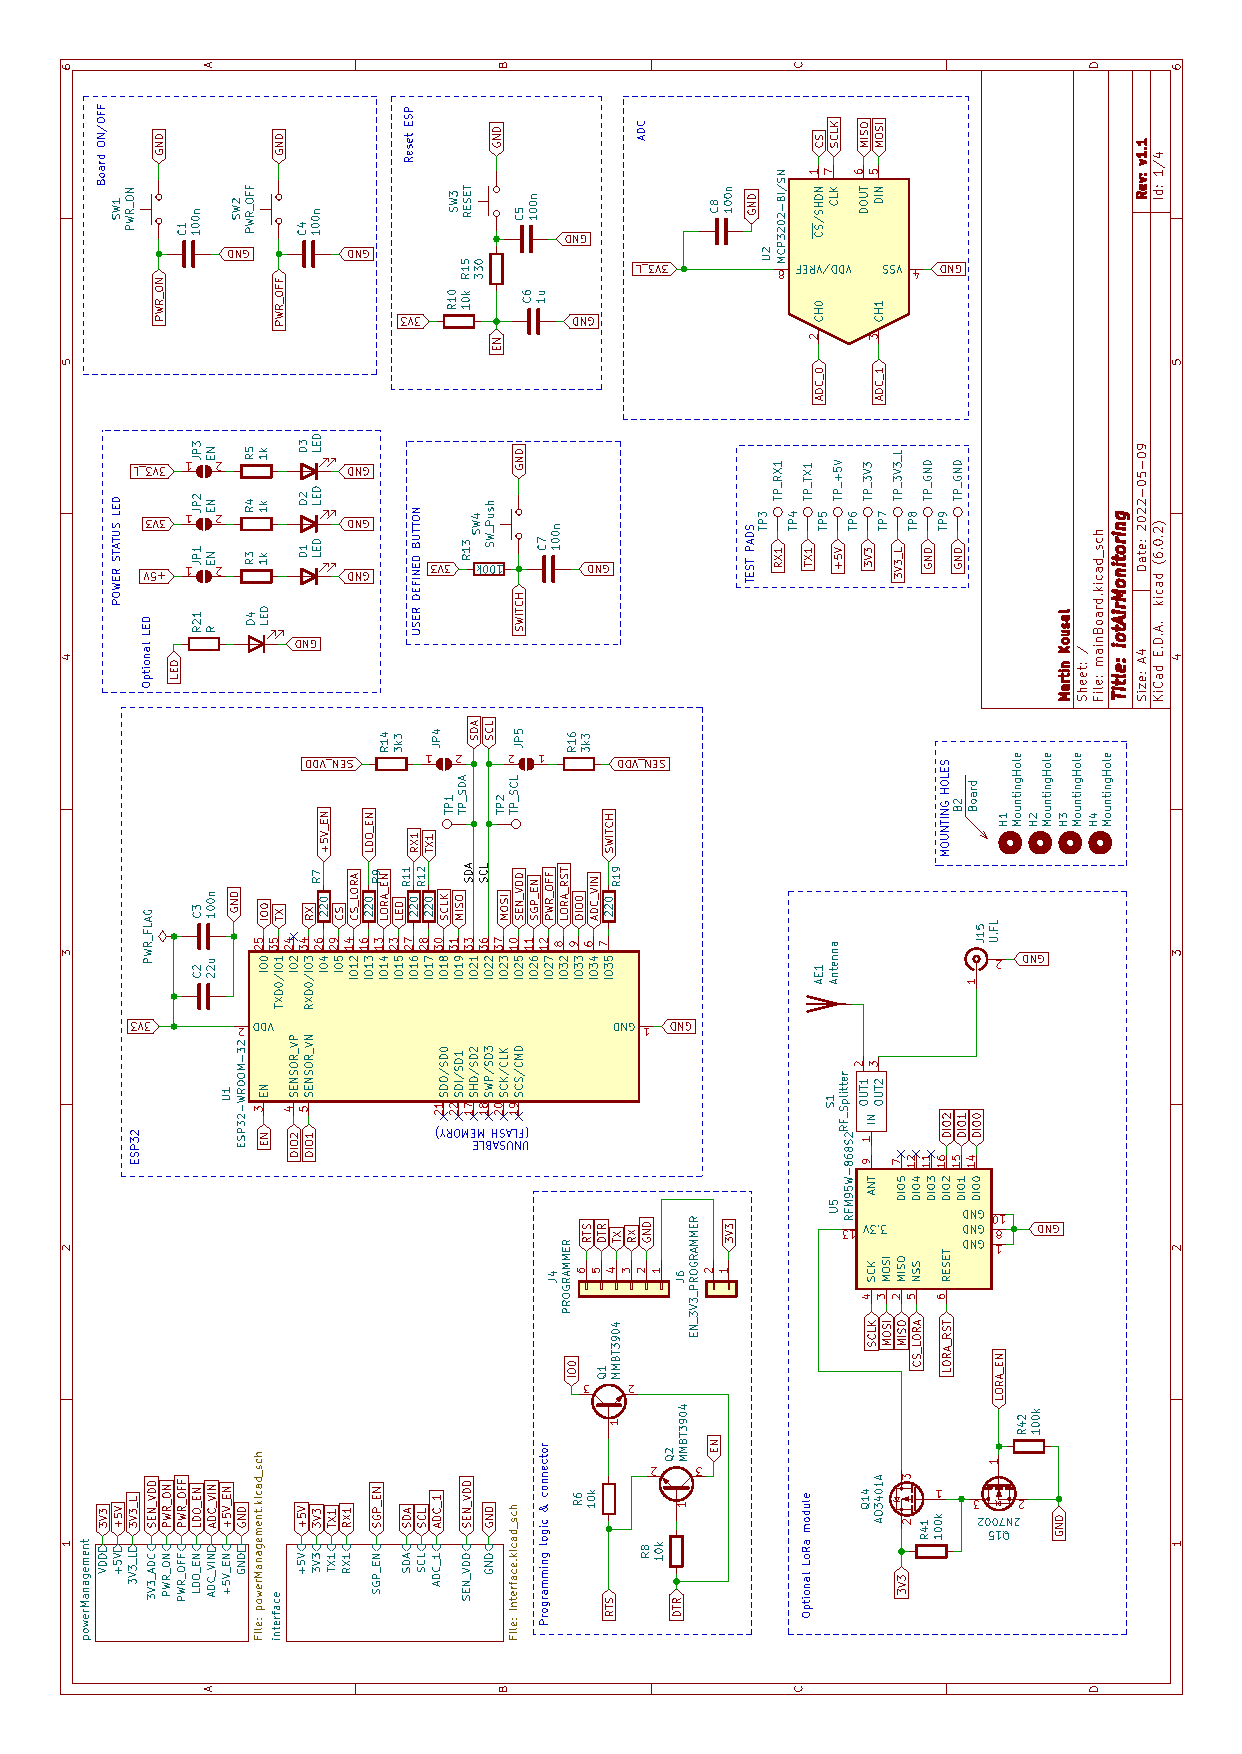
\includepdf[pages=1-]{obrazky/mainBoard.pdf}
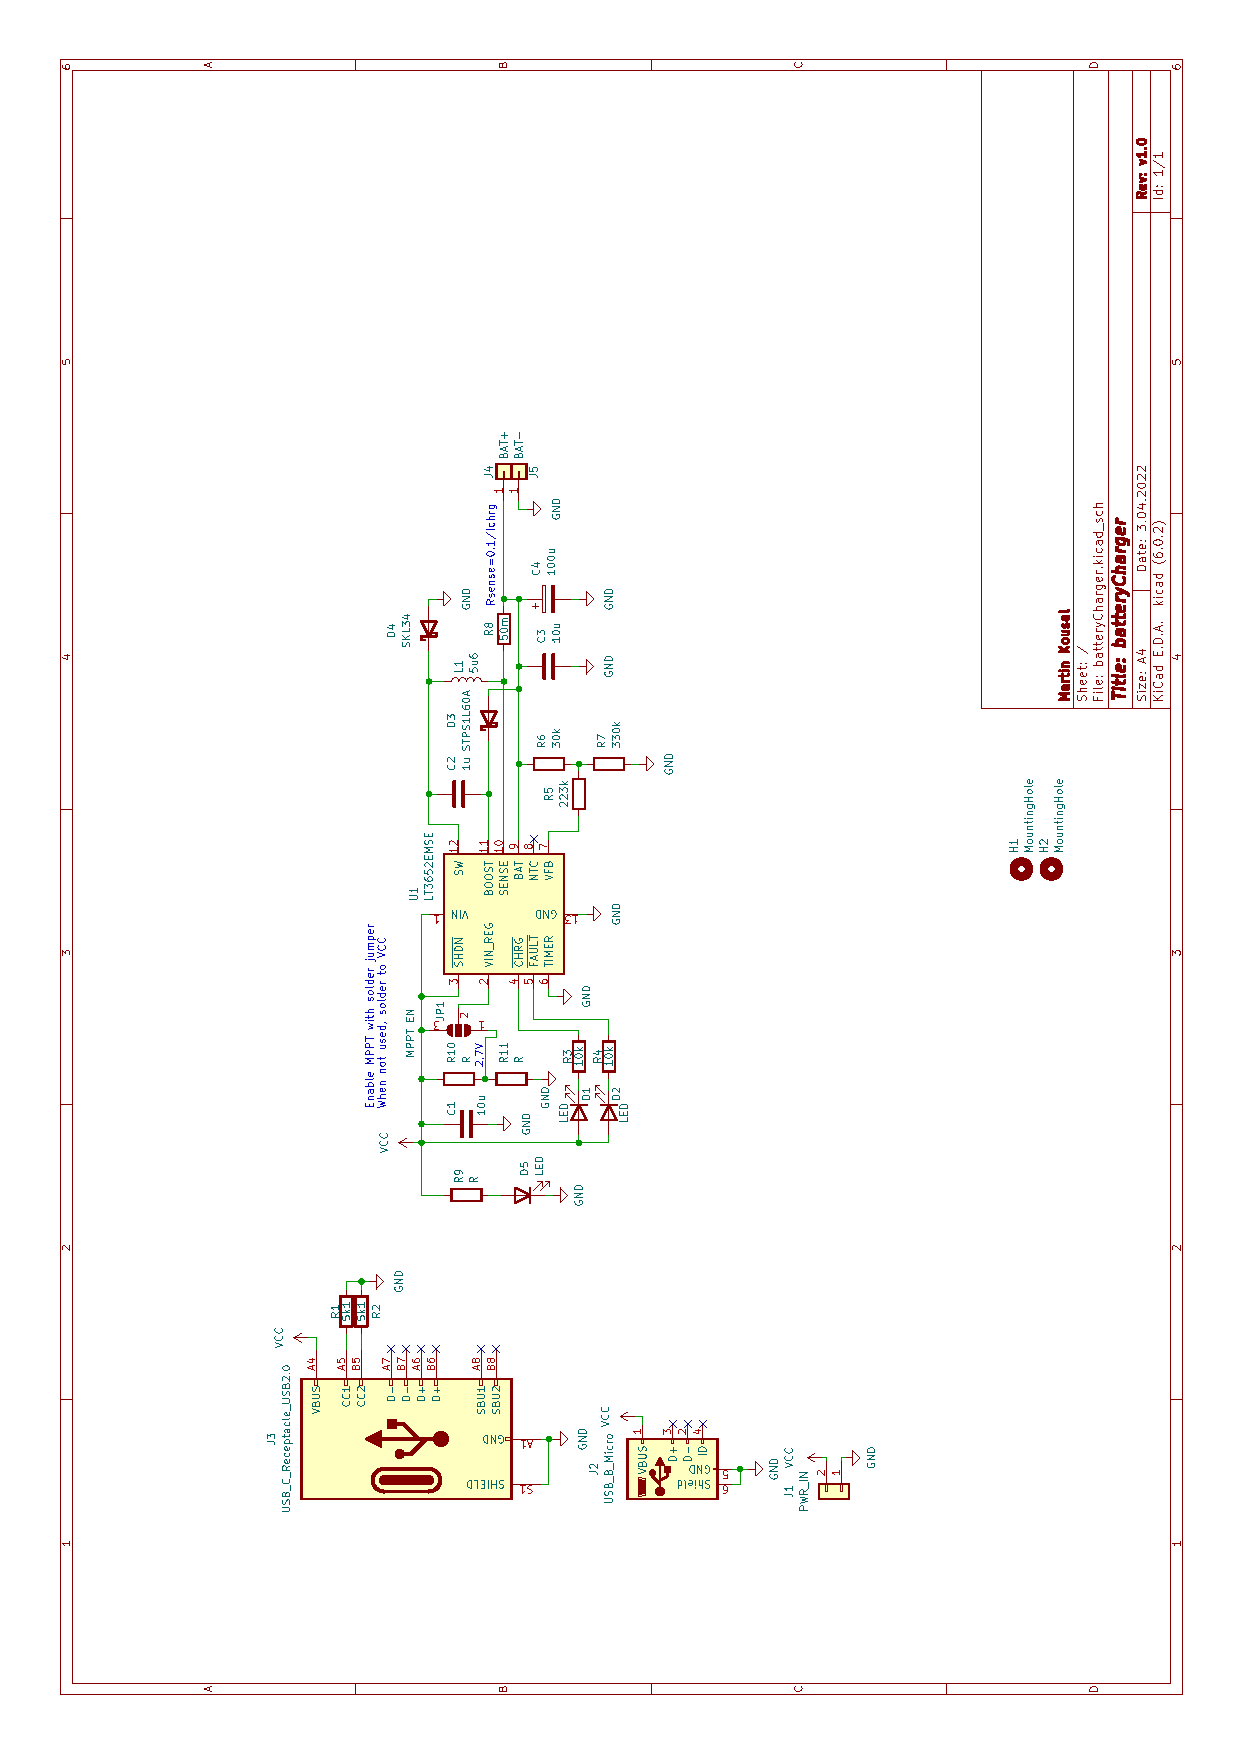
\includepdf[pages=1-]{obrazky/batteryCharger.pdf}

\chapter{Foto realizované desky plošných spojů a zařízení}
\begin{figure}[h]
	\centering
	\subfloat[][Horní strana desky]{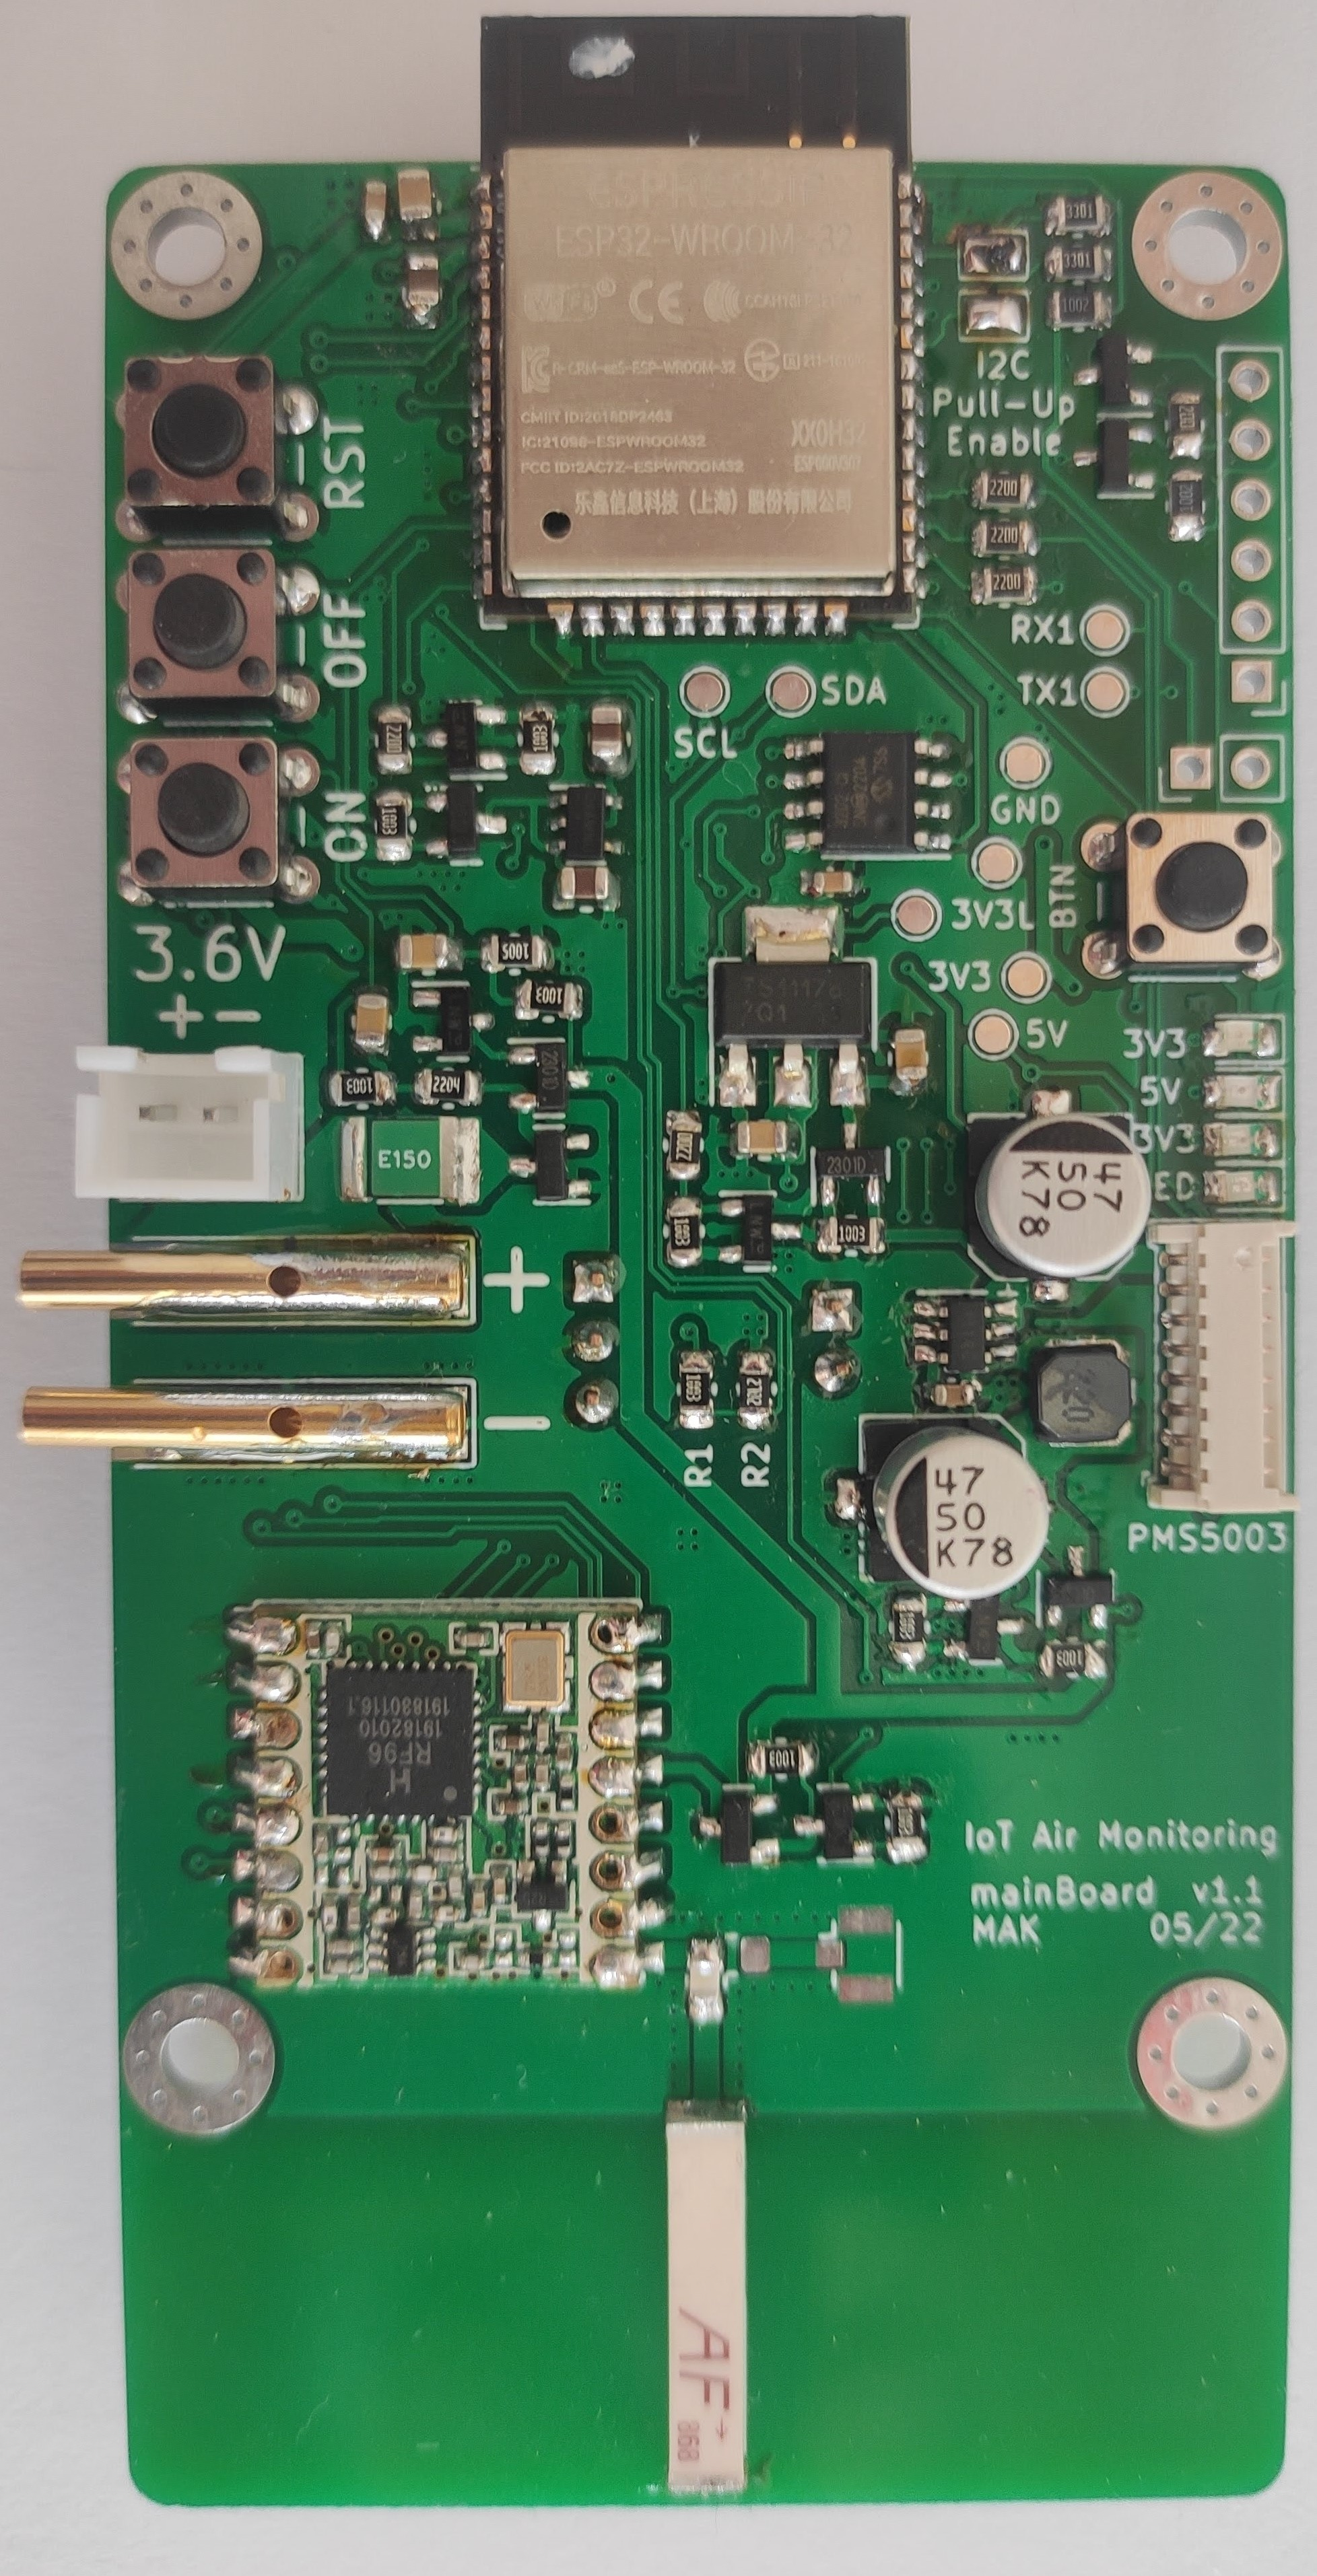
\includegraphics[width=0.48\textwidth]{obrazky/final_pcb_top.jpg}}
	\quad
	\subfloat[][Spodní strana desky]{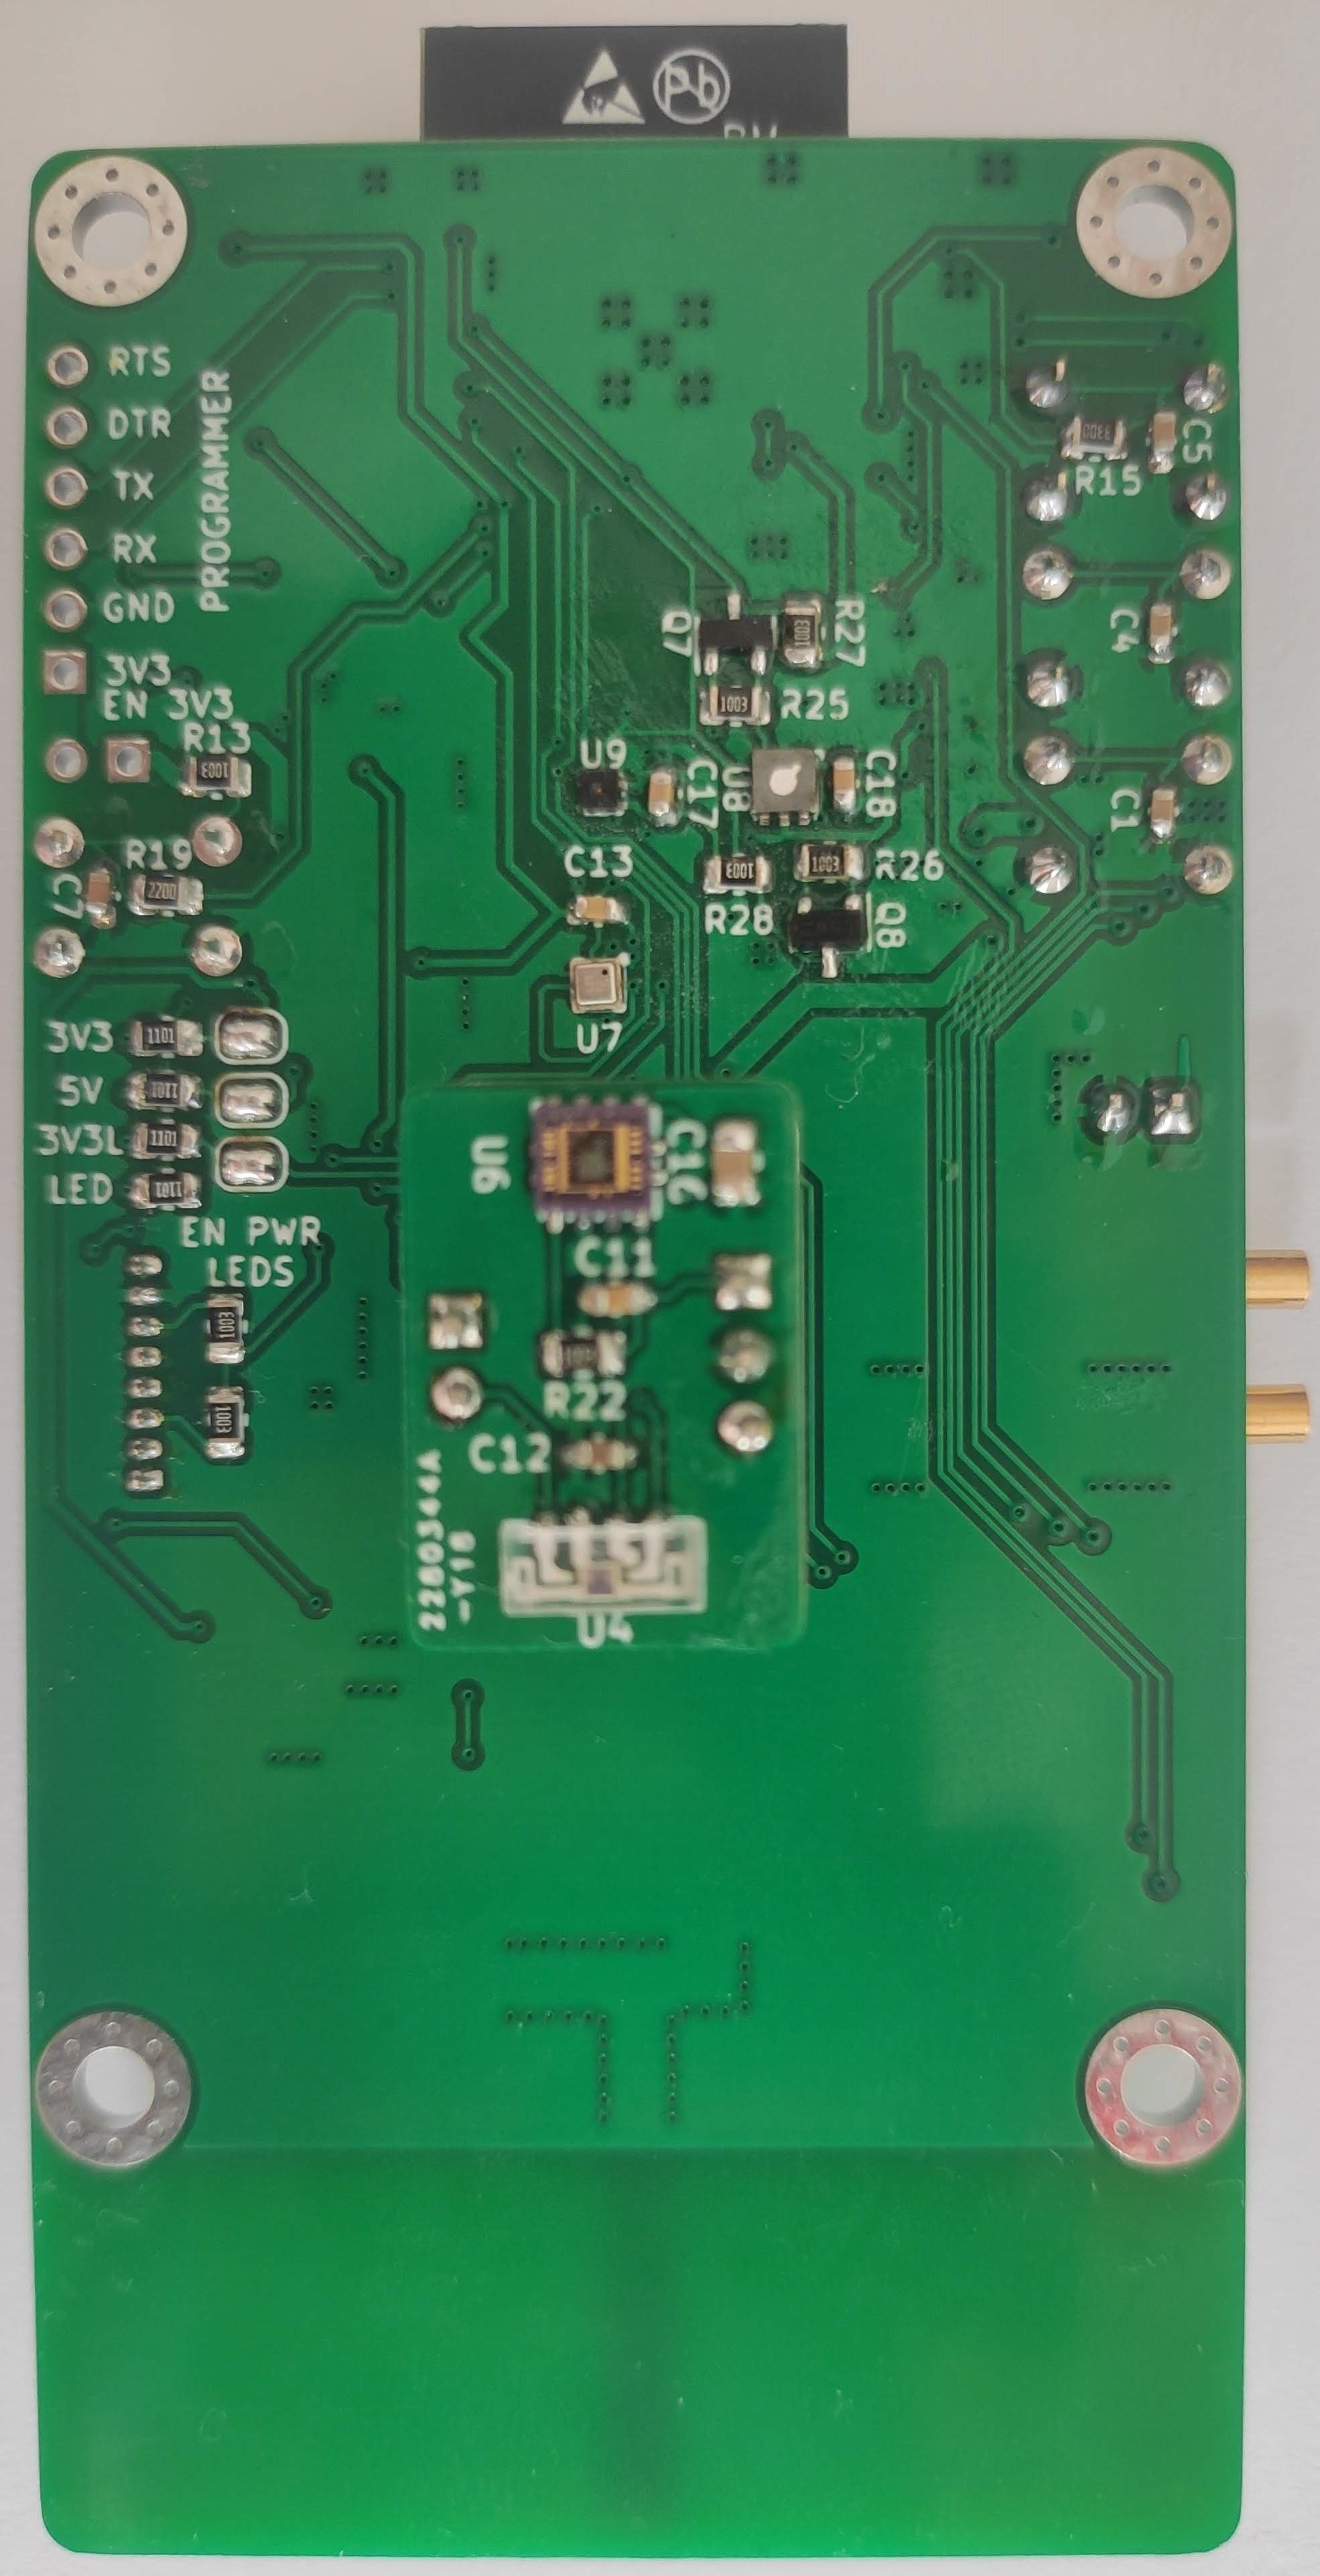
\includegraphics[width=0.48\textwidth]{obrazky/final_pcb_bot.jpg}}
	\caption{Foto osazené desky s elektronikou včetně světelných senzorů.}
	\label{fig_finalPCB}
\end{figure}


\chapter{Seznam použitých součástek}

\begin{table}[!ht]
    \centering
    \begin{tabular}{|l|l|l|l|l|}
    \hline
        AE1,  & 1 & Antenna & Antenna\_1 & mainBoard:ANT-868-CHP-T \\ \hline
        BT1,  & 1 & 18650 holder & Battery\_Cell & Connector\_JST:JST\_XH\_B2B-XH-A\_1x02\_P2.50mm\_Vertical \\ \hline
        C1, C3, C4, C5, C7, C8, C11, C12, C13, C17, C18, C20,  & 12 & 100n & C & Capacitor\_SMD:C\_0603\_1608Metric \\ \hline
        C2, C9, C10, C14, C15,  & 5 & 22u & C & Capacitor\_SMD:C\_0805\_2012Metric \\ \hline
        C6, C22, C23,  & 3 & 1u & C & Capacitor\_SMD:C\_0805\_2012Metric \\ \hline
        C16,  & 1 & 1n & C & Capacitor\_SMD:C\_0805\_2012Metric \\ \hline
        C19, C21,  & 2 & 47u & C\_Polarized & Capacitor\_SMD:CP\_Elec\_6.3x7.7 \\ \hline
        D1, D2, D3, D4,  & 4 & LED & LED & LED\_SMD:LED\_0805\_2012Metric\_Pad1.15x1.40mm\_HandSolder \\ \hline
        F1,  & 1 & Polyfuse & Polyfuse & Fuse:Fuse\_1812\_4532Metric\_Pad1.30x3.40mm\_HandSolder \\ \hline
        H1, H2, H3, H4,  & 4 & MountingHole & MountingHole & MountingHole:MountingHole\_3.2mm\_M3\_Pad\_Via \\ \hline
        J1,  & 1 & PWR\_LIGHT & Conn\_01x03 & Connector\_PinHeader\_2.54mm:PinHeader\_1x03\_P2.54mm\_Vertical \\ \hline
        J2,  & 1 & I2C & Conn\_01x02 & Connector\_PinHeader\_2.54mm:PinHeader\_1x02\_P2.54mm\_Vertical \\ \hline
        J3,  & 1 & PWR\_LIGHT & Conn\_01x03 & Connector\_PinSocket\_2.54mm:PinSocket\_1x03\_P2.54mm\_Vertical \\ \hline
        J4,  & 1 & PROGRAMMER & Conn\_01x06 & Connector\_PinHeader\_2.54mm:PinHeader\_1x06\_P2.54mm\_Vertical \\ \hline
        J5,  & 1 & I2C & Conn\_01x02 & Connector\_PinSocket\_2.54mm:PinSocket\_1x02\_P2.54mm\_Vertical \\ \hline
        J6,  & 1 & EN\_3V3\_PROGRAMMER & Conn\_01x02 & Connector\_PinHeader\_2.54mm:PinHeader\_1x02\_P2.54mm\_Vertical \\ \hline
        J8,  & 1 & PMS5003 & Conn\_01x08 & Connector\_Molex:Molex\_PicoBlade\_53048-0810\_1x08\_P1.25mm\_Horizontal \\ \hline
        J9,  & 1 & BAT- & Conn\_01x01 & mainBoard:2mm\_Banana-Socket \\ \hline
        J10,  & 1 & BAT+ & Conn\_01x01 & mainBoard:2mm\_Banana-Socket \\ \hline
        J15,  & 1 & U.FL & Conn\_Coaxial & Connector\_Coaxial:U.FL\_Hirose\_U.FL-R-SMT-1\_Vertical \\ \hline
        JP1, JP2, JP3,  & 3 & EN & SolderJumper\_2\_Open & Jumper:SolderJumper-2\_P1.3mm\_Open\_RoundedPad1.0x1.5mm \\ \hline
        JP4, JP5,  & 2 & ~ & SolderJumper\_2\_Open & Jumper:SolderJumper-2\_P1.3mm\_Open\_TrianglePad1.0x1.5mm \\ \hline
        L1,  & 1 & 22u & L & Inductor\_SMD:L\_Coilcraft\_LPS4018 \\ \hline
        Q1, Q2,  & 2 & MMBT3904 & Q\_NPN\_BEC & Package\_TO\_SOT\_SMD:SOT-23 \\ \hline
        Q3, Q5, Q9, Q10, Q12, Q14,  & 6 & AO3401A & Q\_PMOS\_GSD & Package\_TO\_SOT\_SMD:SOT-23 \\ \hline
        Q4, Q6, Q7, Q8, Q11, Q13, Q15,  & 7 & 2N7002 & 2N7002 & Package\_TO\_SOT\_SMD:SOT-23 \\ \hline
        R1, R2,  & 2 & R & R & Resistor\_SMD:R\_0805\_2012Metric\_Pad1.20x1.40mm\_HandSolder \\ \hline
        R3, R4, R5,  & 3 & 1k & R & Resistor\_SMD:R\_0805\_2012Metric \\ \hline
        R6, R8, R10,  & 3 & 10k & R & Resistor\_SMD:R\_0805\_2012Metric \\ \hline
        R7, R9, R11, R12, R18, R19,  & 6 & 220 & R & Resistor\_SMD:R\_0805\_2012Metric \\ \hline
        R13, R17, R20, R22, R23, R24, R25, R26, R27, R28, R30, R31, R33, R36, R39, R40, R41, R42,  & 18 & 100k & R & Resistor\_SMD:R\_0805\_2012Metric \\ \hline
        R14, R16,  & 2 & 3k3 & R & Resistor\_SMD:R\_0805\_2012Metric \\ \hline
        R15,  & 1 & 330 & R & Resistor\_SMD:R\_0805\_2012Metric \\ \hline
        R21,  & 1 & R & R & Resistor\_SMD:R\_0805\_2012Metric \\ \hline
        R29,  & 1 & 2M2 & R & Resistor\_SMD:R\_0805\_2012Metric \\ \hline
        R32,  & 1 & 10M & R & Resistor\_SMD:R\_0805\_2012Metric \\ \hline
        S1,  & 1 & RF\_Splitter & RF\_Splitter & mainBoard:RF\_Splitter \\ \hline
        SW1,  & 1 & PWR\_ON & SW\_Push & Button\_Switch\_THT:SW\_PUSH\_6mm \\ \hline
        SW2,  & 1 & PWR\_OFF & SW\_Push & Button\_Switch\_THT:SW\_PUSH\_6mm \\ \hline
        SW3,  & 1 & RESET & SW\_Push & Button\_Switch\_THT:SW\_PUSH\_6mm \\ \hline
        SW4,  & 1 & SW\_Push & SW\_Push & Button\_Switch\_THT:SW\_PUSH\_6mm \\ \hline
        TP1,  & 1 & TP\_SDA & TestPoint & TestPoint:TestPoint\_Pad\_D1.5mm \\ \hline
        TP2,  & 1 & TP\_SCL & TestPoint & TestPoint:TestPoint\_Pad\_D1.5mm \\ \hline
        TP3,  & 1 & TP\_RX1 & TestPoint & TestPoint:TestPoint\_Pad\_D1.5mm \\ \hline
        TP4,  & 1 & TP\_TX1 & TestPoint & TestPoint:TestPoint\_Pad\_D1.5mm \\ \hline
        TP5,  & 1 & TP\_+5V & TestPoint & TestPoint:TestPoint\_Pad\_D1.5mm \\ \hline
        TP6,  & 1 & TP\_3V3 & TestPoint & TestPoint:TestPoint\_Pad\_D1.5mm \\ \hline
        TP7,  & 1 & TP\_3V3\_L & TestPoint & TestPoint:TestPoint\_Pad\_D1.5mm \\ \hline
        TP8, TP9,  & 2 & TP\_GND & TestPoint & TestPoint:TestPoint\_Pad\_D1.5mm \\ \hline
        U1,  & 1 & ESP32-WROOM-32 & ESP32-WROOM-32 & RF\_Module:ESP32-WROOM-32 \\ \hline
        U2,  & 1 & MCP3202-BI/SN & MCP3202 & Package\_SO:SOIC-8\_3.9x4.9mm\_P1.27mm \\ \hline
        U3,  & 1 & AMS1117-3.3 & AMS1117-3.3 & Package\_TO\_SOT\_SMD:SOT-223-3\_TabPin2 \\ \hline
        U4,  & 1 & VEML7700 & VEML7700 & mainBoard:VEML7700 \\ \hline
        U5,  & 1 & RFM95W-868S2 & RFM95W-868S2 & RF\_Module:HOPERF\_RFM9XW\_SMD \\ \hline
        U6,  & 1 & ML8511 & ML8511 & mainBoard:ML8511 \\ \hline
        U7,  & 1 & BMP388 & BMP388 & mainBoard:BMP388 \\ \hline
        U8,  & 1 & SGP30 & SGP30 & mainBoard:SGP30 \\ \hline
        U9,  & 1 & SHT40 & SHT40 & mainBoard:SHT40 \\ \hline
        U10,  & 1 & AP1603 & AP1603 & Package\_TO\_SOT\_SMD:SOT-23-6\_Handsoldering \\ \hline
        U11,  & 1 & NCP115ASN180T2G & NCP115ASN180T2G & Package\_SO:TSOP-5\_1.65x3.05mm\_P0.95mm \\ \hline
    \end{tabular}
\end{table}


\chapter{Obsah elektronické přílohy}

{\small
\dirtree{%
.1 /.
.2 hw\DTcomment{Podklady pro PCB}.
}
}